
\section{The OSSolverService}\label{section:ossolverservice}

The {\tt OSSolverService}\index{OSSolverService@{\tt OSSolverService}|(} is a command line executable designed
to pass problem instances in either  OSiL\index{OSiL}, AMPL nl\index{AMPL nl format}, or MPS format\index{MPS format}
to solvers and get the optimization result back to be displayed either to standard output or a specified browser.
The {\tt OSSolverService} can be used to invoke a solver locally or on a remote server. It can communicate with a remote solver both synchronously and asynchronously.
%It can work either synchronously or asynchronously. 
At present six service methods are implemented, 
{\tt solve}\index{solve@{\tt solve}},
{\tt send}\index{send@{\tt send}}, 
{\tt retrieve}\index{retrieve@{\tt retrieve}},
{\tt getJobID}\index{getJobID@{\tt getJobID}}, 
{\tt knock}\index{knock@{\tt knock}} and 
{\tt kill}\index{kill@{\tt kill}}.
These methods are explained in more detail in Section~\ref{section:servicemethods}. Only the {\tt solve} method is available locally. 

There are two ways  to use the {\tt OSSolverService} executable. The first way
is to use the interactive shell. The interactive shell is invoked by either 
double clicking on the icon for the {\tt OSSolverService} executable, or by opening a command
window, connecting to the directory holding the executable, and then typing in
{\tt OSSolverService} with no arguments. Using the interactive shell is fairly
intuitive and we do not discuss in detail. The second way to use the {\tt
OSSolverService} executable is to provide arguments at the command line. This is
discussed next. The command line arguments are also valid for the interactive shell. 

\subsection{OSSolverService Input Parameters}\label{section:OSSolverServiceInputParameters}

At present, the {\tt OSSolverService} takes the following parameters. The order of the parameters is irrelevant.
Not all the parameters are required. 
%However, if the {\tt solve}\index{solve@{\tt solve}} or {\tt send}\index{send@{\tt send}} service    
%methods  (see Section~\ref{section:servicemethods} ) are invoked a problem instance location must be specified.

\begin{itemize}


\item[] {\bf osil xxx.osil}\ \ This is the path information and name of
the file that contains the optimization instance in OSiL\index{OSiL} format.
It is assumed that this file is available on the machine that is running
{\tt OSSolverService}. This parameter can be omitted, as there are other ways
to specify an optimization instance.
%If this option is not specified then the instance location must be specified in the OSoL\index{OSoL} solver options file.

\item[] {\bf osol xxx.osol}\ \ This is the path information and name of the file that contains the solver 
options. It is assumed that this file is available on the machine that is running {\tt OSSolverService}. 
It is not necessary to specify this parameter.

\item[] {\bf osrl xxx.osrl}\ \ This is the path information and name of the file to which the solver 
solution will be written upon return. A valid file path must be given on the machine that is running {\tt OSSolverService}. 
It is not necessary to specify this parameter.
If this parameter is not specified then the solver solution is displayed to the screen.


\item[] {\bf osplInput xxx.ospl}\ \  The name of an input file in the  OS Process Language (OSpL); 
this is used as input  to the {\tt knock} method.

\item[] {\bf osplOutput xxx.ospl}\ \  The name of an output file in the  OS Process Language (OSpL); 
this is the  output  string from the {\tt knock}  and {\tt kill} method.

\item[] {\bf serviceLocation url}\ \ This is the URL of the solver service.
It is not required, and if not specified it is assumed that the problem
is solved locally.

\item[] {\bf serviceMethod  methodName}\ \ This is  the method on the solver service to be invoked.
The options are 
{\tt solve}\index{solve@{\tt solve}|(}, 
{\tt send}\index{send@{\tt send}},
{\tt kill}\index{kill@{\tt kill}}, 
{\tt knock}\index{knock@{\tt knock}},
{\tt getJobID}\index{getJobID@{\tt getJobID}}, and 
{\tt retrieve}\index{retrieve@{\tt retrieve}}.
The use of these options is illustrated in the examples below. This parameter is not required, 
and the default value is {\tt solve}\index{solve@{\tt solve}|)}.

\item[] {\bf mps  xxx.mps}\ \ This is the path information and name of the MPS file if the problem instance 
is in MPS format\index{MPS format}. It is assumed that this file is available on the machine that is running 
{\tt OSSolverService}. The default file format is OSiL\index{OSiL} so this option is not required.

\item[] {\bf nl  xxx.nl}\ \ This is the path information and name of the AMPL nl file if the problem instance 
is in AMPL nl format\index{AMPL nl format}. It is assumed that this file is available on the machine that is running
{\tt OSSolverService}. The default file format is OSiL\index{OSiL} so this option is not required.

\item[] {\bf solver  solverName}\ \ {\bf Note that this option only has effect for local calls.} 
For a remote solve or send, put the solver name into the field {\tt <solverToInvoke>} in an
OSoL file and specify this file with {\tt osol ...}.
%Possible values for default OS installation are {\tt clp} (COIN-OR Clp),
%{\tt cbc} (COIN-OR Cbc), {\tt dylp} (COIN-OR DyLP), and {\tt symphony} (COIN-OR SYMPHONY).
Possible values of this parameter depend on the installation. The default configurations can be read off from
Table~\ref{table:configurations}.
Other solvers supported (if the necessary libraries are present) are 
{\tt cplex} (Cplex through COIN-OR Osi)\index{cplex@{\tt cplex}}\index{COIN-OR projects!Osi@{\tt Osi}|(},
{\tt glpk} (GLPK\index{Third-party software, {\tt GLPK}} through COIN-OR Osi\index{COIN-OR projects!Osi@{\tt Osi}|)})
%, {\tt ipopt} (COIN-OR Ipopt)
\ifknitro, {\tt knitro} (Knitro)\index{Knitro@{\tt Knitro}}\fi
and {\tt lindo} (LINDO)\index{LINDO}.
If no value is specified for this parameter, then a default solver is used 
%then {\tt cbc}\index{COIN-OR projects!Cbc@{\tt Cbc}} is the default value of this parameter 
for the {\tt solve}\index{solve@{\tt solve}} or {\tt send}\index{send@{\tt send}} service method.
The default solver depends on the problem type and can be read off from 
table~\ref{table:defaultsolvers}.\index{default solver}


\begin{table}
\caption{Solver configurations}
\centering
\label{table:configurations}
\vskip 8pt
 \begin{tabular}{l|c|c|c|}
 & {binaries} & {UNIX build} & {MSVS build} \\
 & (Section~\ref{section:obtainingbinaries})
 & (Section~\ref{section:unixbuilds})
 & (Section~\ref{section:windowsinstall})\\ \hline
Bonmin   & x & x$^1$ & x$^{1,2}$ \\
Cbc      & x & x     & x \\
Clp      & x & x     & x \\
Couenne  & x & x$^1$ & --- \\
DyLP     & x & x     & --- \\
Ipopt    & x & x$^1$ & x$^{1,2}$ \\
SYMPHONY & x & x     & x \\
Vol      & x & x     & x \\ \hline
\end{tabular}
\vskip 6pt
\begin{tabular}{l}
Explanations:\\
$\qquad{}^1$Requires third-party software to be downloaded\\
$\qquad{}^2$Requires Fortran compiler (see Section~\ref{section:ipopt})
\end{tabular}
\end{table}\index{supported solvers}

\begin{table}
\caption{Default solvers}
\centering
\label{table:defaultsolvers}\index{default solver}
\vskip 8pt
\begin{tabular}{l|c}
Problem type & Default solver \\ \hline
Linear, continuous   & Clp \\
Linear, integer      & Cbc \\
Nonlinear, continuous& Ipopt \\ 
Nonlinear, integer   & Bonmin \\ \hline
\end{tabular}
\end{table}


\item[] {\bf browser  browserName}\ \ This parameter is a path to the browser on the local machine. 
If this optional parameter is specified then the solver result in OSrL\index{OSrL} format is transformed 
using XSLT into HTML and displayed in the browser.

\item[] {\bf config pathToConfigureFile}\ \ This optional parameter specifies a path on the local machine 
to a text file containing values for the input parameters. This is convenient for the user not wishing 
to constantly retype parameter values.

\item[] {\bf -help}\ \  This parameter prints out the list of available options (in essence, this list).
Synonyms for {\bf -help} are {\bf -h} and {\bf -?}.

\item[] {\bf -version}\ \ This parameter prints version and licence information. {\bf -v} is an acceptable synonym.

\end{itemize}



The input parameters to the {\tt OSSolverService} may be given entirely in the command line or in a configuration file.
We first illustrate giving all the  parameters in the command line. The following command will invoke the
{\tt Clp}\index{COIN-OR projects!Clp@{\tt Clp}} solver on the local machine to solve the problem instance
{\tt parincLinear.osil}\index{parincLinear.osil@{\tt parincLinear.osil}|(}.
When invoking the commands below involving {\tt OSSolverService} we assume that
1) the user is connected to the directory where the {\tt OSSolverService} executable is located, and
2) that {\tt ../data/osilFiles} is a valid path to {\tt COIN-OS/data/osilFiles}.  If the OS project was built successfully,
then there is a copy of  {\tt OSSolverService} in {\tt COIN-OS/OS/src}. The user may wish to execute {\tt OSSolverService}
from this {\tt src} directory so that all that follows is correct in terms of path definitions.


\begin{verbatim}
./OSSolverService solver clp osil ../data/osilFiles/parincLinear.osil
\end{verbatim}

Alternatively, these parameters can be put into a configuration file.
Assume that the configuration file of interest is {\tt testlocalclp.config}.
It would contain the two lines of information
\begin{verbatim}
osil ../data/osilFiles/parincLinear.osil
solver clp
\end{verbatim}
\index{parincLinear.osil@{\tt parincLinear.osil}|)}
Then the command line is
\begin{verbatim}
./OSSolverService config ../data/configFiles/testlocalclp.config
\end{verbatim}

{\bf Windows users} should {\bf note} that the folder separator is always 
the forward slash (`/') instead of the customary backslash (`$\backslash$').


Parameters specified in the configure file are overridden by parameters specified at the command line.
This is convenient if a user has a base configure file and wishes to override only a few options. For example,
\begin{verbatim}
./OSSolverService config ../data/configFiles/testlocalclp.config solver lindo
\end{verbatim}
or
\begin{verbatim}
./OSSolverService solver lindo config ../data/configFiles/testlocalclp.config
\end{verbatim}
will result in the LINDO\index{LINDO} solver being used even though {\tt Clp}\index{COIN-OR projects!Clp@{\tt Clp}} is specified in the
{\tt testlocalclp} configure file.

Some things to note:

\begin{enumerate}
\item{}  The default {\tt serviceMethod} is {\tt solve} if another service method is not specified.
The service method cannot be specified in the OSoL options file.

\item{} The command line parameters are intended to only influence the behavior of the local {\tt OSSolverService}. 
In particular, only the service method is transmitted to a remote location. Any communication with a remote solver other than setting the service method {\bf must} take place through an OSoL options file.
   
\item{}  Only the {\tt solve()} method is available for local calls
to {\tt OSSolverService}.

\item{}  If the options {\tt send}\index{send@{\tt send}}, {\tt kill}\index{kill@{\tt kill}},
{\tt knock}\index{knock@{\tt knock}},  {\tt getJobID}\index{getJobID@{\tt getJobID}},
or {\tt retrieve}\index{retrieve@{\tt retrieve}} are specified,
a  {\tt serviceLocation}\index{serviceLocation@{\tt serviceLocation}} must be specified.

\item{}  When using the {\tt send()}\index{send@{\tt send}} or  {\tt solve()}\index{solve@{\tt solve}} methods
a problem instance must be specified.

\end{enumerate}


\subsection{The Command Line Parser}\label{section:commandlineparser}

The top layer of the local OSSolverService is a command line parser that parses the command line and
the config file (if one is specified) and passes the information on to a local solver or a remote solver service,
depending on whether a {\tt serviceLocation} was specified. If a 
{\tt serviceLocation} is specified a call is made to a remote solver service, otherwise a local solver is called.

\medskip

If a local solve is indicated, we pass to a solver in the OSLibrary two things: 
an OSoL file if one has been specified and a problem instance. The problem instance 
is the instance in the OSiL file specified by the {\tt osil} option. If there is no OSiL file, 
then it is the instance specified in the nl file. If there is no nl file, it is the 
instance in the mps file. If no OSiL, nl or mps file is specified, an error is thrown. 

The OSoL file is simply passed on to the OSLibrary; it is not parsed at this point. 
The OSoL file elements {\tt <solverToInvoke>} and {\tt <instanceLocation>} cannot be used for local calls.
One can specify which solver to use in the OSLibrary through the {\tt solver} option. If this 
option is empty, a default solver is selected (see Table~\ref{table:defaultsolvers}\index{default solver}).

\medskip

If the {\tt serviceLocation} parameter is used, a call is placed to the remote solver service
specified in the {\tt serviceLocation} parameter. 
Two strings are passed to the remote solver service: a string which is the OSoL file 
if one has been specified, or the empty string otherwise, and a string containing an 
instance if one has been specified. The instance can be specified using the {\tt osil}, {\tt nl}, or 
{\tt mps} option. If an OSiL file is specified in the {\tt osil} option, it is used. If there is no 
OSiL file, then the instance specified in the nl file is used. If there is no nl file,  
the mps file is used. If no file is given, an empty string is sent.

For remote calls, the solver can only be set in the osol file, using the element {\tt <solverToInvoke>};
the {\tt solver} option has no effect.



\subsection{Solving Problems Locally}

Generally, when solving a problem locally the user will use the {\tt solve}\index{solve@{\tt solve}} service 
method. The {\tt solve} method is invoked synchronously and waits for the solver to return the result.  
This is illustrated in Figure~\ref{figure:ossolverservicelocal}. As illustrated, the {\tt OSSolverService} 
reads a file on the hard drive with the optimization instance, usually in OSiL\index{OSiL} format. 
The optimization instance is parsed into a string which is passed to the {\tt OSLibrary}\index{OSLibrary@{\tt OSLibrary}} 
(see Section~\ref{section:oslibrary}), which is linked with various solvers. 
Similarly an option file in OSoL\index{OSoL} format is parsed into a string and passed to the {\tt OSLibrary}. 
{\it No interpretation of the options is done at this stage}, so that any {\tt <solverToInvoke>} or
{\tt <instanceLocation>} directives in the OSoL file will be ignored for local solves.
The result of the optimization is passed back to the {\tt OSSolverService} as a string in OSrL\index{OSrL} format.



\begin{figure}
\centering
%\includegraphics[scale=0.5]{\figurepath/OSSolverServiceLocal.png}
%\includegraphics[scale=0.5]{./figures/OSSolverServiceLocal.png}
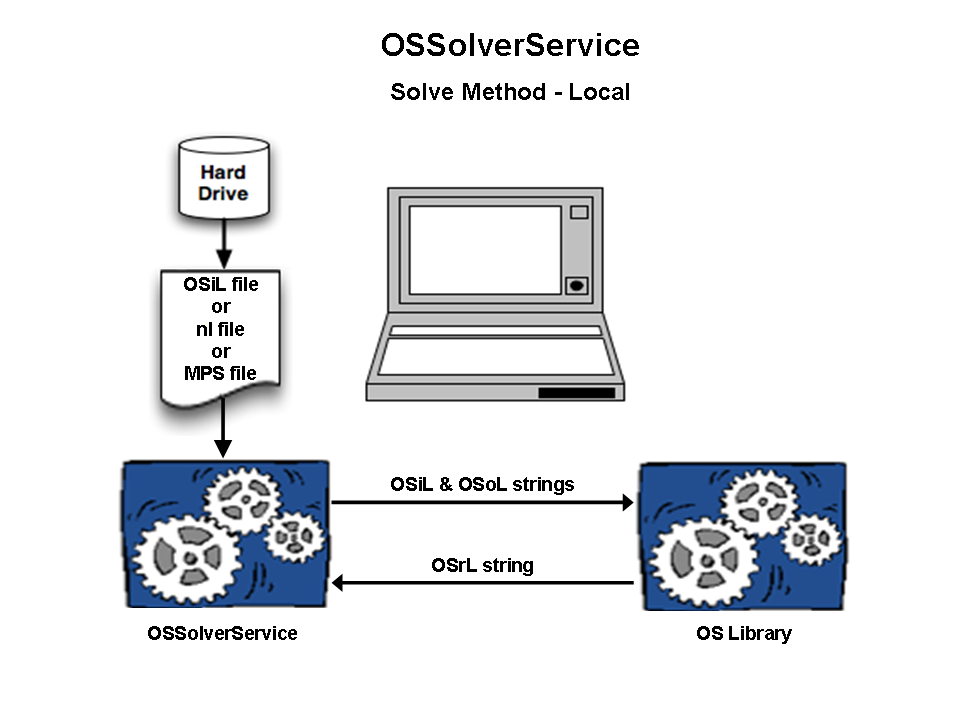
\includegraphics[scale=0.5]{./figures/Figure9.png}
\caption{A local call to {\tt solve}.}
\label{figure:ossolverservicelocal}
\end{figure}



Here is an example of using a configure file,  {\tt testlocal.config}\index{testlocal.config@{\tt testlocal.config}|(},
to invoke {\tt Ipopt}\index{COIN-OR projects!Ipopt@{\tt Ipopt}} locally using the {\tt solve}\index{solve@{\tt solve}} command.

\begin{verbatim}
osil ../data/osilFiles/parincQuadratic.osil
solver ipopt
serviceMethod solve
browser /Applications/Firefox.app/Contents/MacOS/firefox
osrl /Users/kmartin/temp/test.osrl
\end{verbatim}



The first line of {\tt testlocal.config}\index{testlocal.config@{\tt testlocal.config}|)} gives the local location
of the OSiL file,
{\tt parincQuadratic.osil}, that contains the problem instance. The second parameter,
{\tt solver ipopt},  is the solver to be invoked, in this case COIN-OR Ipopt.
The third parameter {\tt serviceMethod solve} is not really needed, since the default solver service 
is {\tt solve}. It is included only for illustration. 
The fourth parameter is the location of the browser on the local machine. 
The fifth parameter is  {\tt osrl}. The value of this parameter, {\tt /Users/kmartin/temp/test.osrl}, 
specifies the location on the local machine where the OSrL\index{OSrL} result file will get written.


%Parameters may also be contained in an XML-file in OSoL\index{OSoL} format. In the configuration %file
%{\tt testlocalosol.config} we illustrate specifying the instance location in an OSoL file.
%\begin{verbatim}
%osol ../data/osolFiles/demo.osol
%solver clp
%\end{verbatim}
%The file {\tt demo.osol} is
%
%\begin{verbatim}
%<?xml version="1.0" encoding="UTF-8"?>
%<osol xmlns="os.optimizationservices.org"
%      xmlns:xsi="http://www.w3.org/2001/XMLSchema-instance"
%      xsi:schemaLocation="os.optimizationservices.org
%      http://www.optimizationservices.org/schemas/2.0/OSiL.xsd">
%    <general>
%        <instanceLocation locationType="local">
%            ../data/osilFiles/parincLinear.osil
%        </instanceLocation>
%    </general>
%</osol>
%\end{verbatim}


\subsection{Solving Problems Remotely with Web Services}\label{section:servicemethods}

In many cases the client machine may be a ``weak client'' and  using a more powerful machine to solve a
hard optimization instance is required. Indeed, one of the major purposes of Optimization Services is to
facilitate optimization in a distributed environment.   We now provide examples that illustrate using the
{\tt OSSolverService} executable to call a remote solver service.   By remote solver service we mean a
solver service that is called using Web Services.  The OS implementation  of the solver service
uses Apache Tomcat\index{Apache Tomcat}. See \url{tomcat.apache.org}. The Web Service running on the server
is a Java program based on Apache Axis\index{Apache Axis}. See \url{ws.apache.org/axis}. This is described
in greater detail in Section~\ref{section:tomcat}.
This Web Service is called {\tt OSSolverService.jws}\index{OSSolverService.jws@{\tt OSSolverService.jws}}.
It is not necessary to use the Tomcat/Axis combination.



See Figure~\ref{figure:ossolverservice} for an illustration of this process.
The client machine uses {\tt OSSolverService} executable to call one of the
six service methods, e.g., {\tt solve}\index{solve@{\tt solve}}. 
The  information such as the problem
instance in OSiL\index{OSiL} format and solver options in OSoL\index{OSoL} format are packaged into
a SOAP\index{SOAP protocol} envelope and sent to the server. The server is running the Java Web
Service {\tt OSSolverService.jws}. This Java program running in the Tomcat
Java Servlet container implements the six service methods. If a {\tt solve}
or {\tt send} request is sent to the server from the client, an optimization
problem must be solved. The Java solver service solves the optimization instance
by  calling the  {\tt OSSolverService} on the server. So there is an {\tt OSSolverService}
on the client that calls the Web Service {\tt  OSSolverService.jws} that in turn
calls  the executable {\tt OSSolverService} on the server.
The Java solver service passes options to the server's {\tt OSSolverService}
%such as where the OSiL file is located and where to write the solution result.
in form of two strings, an osil string representing the instance and an osol string
representing the options (if any). 


For remote calls the instance location can be specified either as a command parameter 
(on the command line or in a config file)
or through the {\tt <instanceLocation>} element in the OSoL\index{OSoL} options file.
OSiL files specified in the {\tt <instanceLocation>} element must be converted to an osil string
by the solver service.
If two instance files
are specified in this way --- one through the local command interface, the other in an options file --- 
the information on the command line takes precedent.
%the solver service is free to pick which one to choose.





\begin{figure}
\centering
%\includegraphics[scale=0.5]{\figurepath/OSSolverService.png}
%\includegraphics[scale=0.5]{./figures/OSSolverService.png}
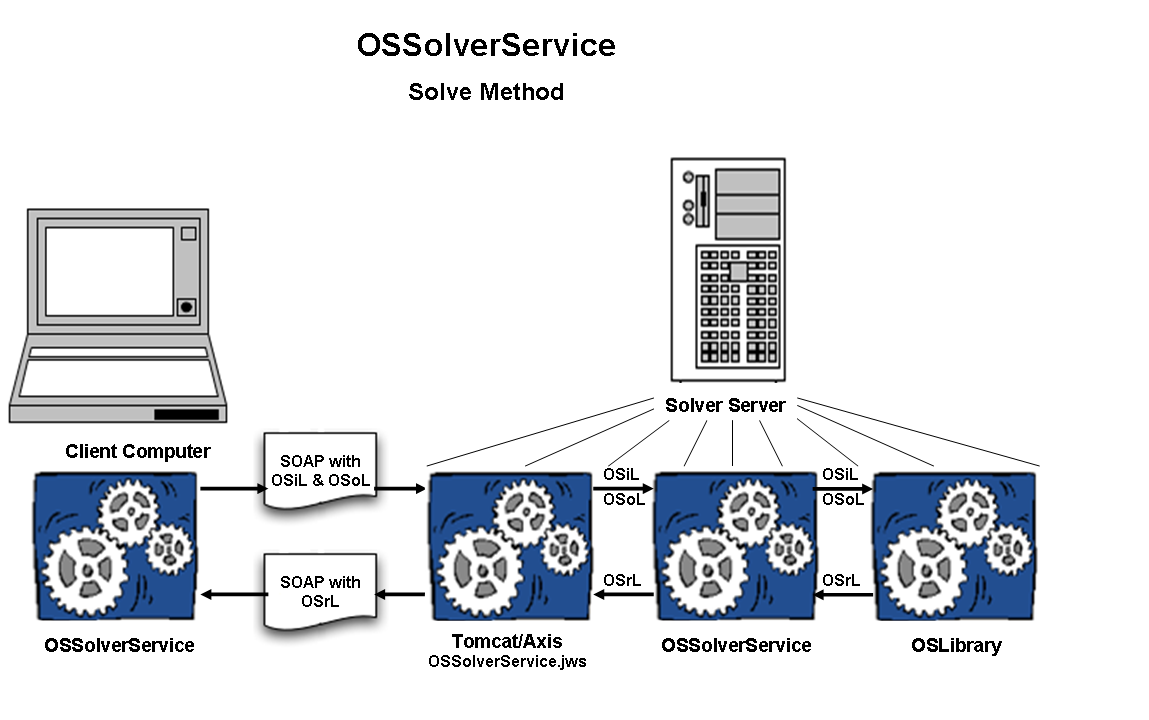
\includegraphics[scale=0.5]{./figures/Figure10.png}
\caption{A remote call to {\tt solve}.}
\label{figure:ossolverservice}
\end{figure}


In the following sections we illustrate each of the six service methods.

\subsubsection{The  {\tt solve} Service Method}\label{section:solve}

\index{solve@{\tt solve}|(}
First we illustrate a simple call to  {\tt OSSolverService.jws}.  The call on the client machine is
\index{testremote.config@{\tt testremote.config}|(}
\begin{verbatim}
./OSSolverService config ../data/configFiles/testremote.config
\end{verbatim}
where the {\tt testremote.config} file is
\begin{verbatim}
osil ../data/osilFiles/parincLinear.osil
serviceLocation http://kipp.chicagobooth.edu/os/OSSolverService.jws
\end{verbatim}

No solver is specified and by default the  {\tt Clp} solver  is used by the {\tt OSSolverService}, 
since the problem is a continuous linear program.
If, for example, the user wished to solve the problem with the 
{\tt SYMPHONY}\index{COIN-OR projects!SYMPHONY@{\tt SYMPHONY}|(} solver then this is accomplished
either by using the  {\tt solver} option on the command line
\begin{verbatim}
./OSSolverService config ../data/configFiles/testremote.config solver symphony
\end{verbatim}
or by  adding  the line
\begin{verbatim}
 solver symphony
\end{verbatim}
to the  {\tt testremote.config} file\index{testremote.config@{\tt testremote.config}|)}.
\index{COIN-OR projects!SYMPHONY@{\tt SYMPHONY}|)}
When solver information is given both on the command line and in the config file, the command line information supercedes the config file.

\index{remoteSolve1.osol@{\tt remoteSolve1.osol}|(}
Next we illustrate a call to the remote SolverService and specify an OSiL instance that is actually residing
on the remote machine that is hosting the {\tt OSSolverService} and not on the client machine.
\begin{verbatim}
./OSSolverService osol ../data/osolFiles/remoteSolve1.osol
     serviceLocation  http://kipp.chicagobooth.edu/os/OSSolverService.jws
\end{verbatim}
where the {\tt remoteSolve1.osol} file is
\begin{verbatim}
<?xml version="1.0" encoding="UTF-8"?>
<osol xmlns="os.optimizationservices.org"
      xmlns:xsi="http://www.w3.org/2001/XMLSchema-instance"
      xsi:schemaLocation="os.optimizationservices.org
      http://www.optimizationservices.org/schemas/2.0/OSiL.xsd">
    <general>
        <instanceLocation locationType="local">c:\parincLinear.osil</instanceLocation>
        <contact transportType="smtp">kipp.martin@chicagogsb.edu</contact>
        <solverToInvoke>ipopt</solverToInvoke>      
    </general>
</osol>
\end{verbatim}
\index{remoteSolve1.osol@{\tt remoteSolve1.osol}|)}

If we were to change the {\tt locationType} attribute in the {\tt <instanceLocation>} element to {\tt http} then we
could specify the instance location on yet another machine. This is illustrated below  for {\tt remoteSolve2.osol}.
The scenario is depicted in Figure~\ref{figure:ossolverservice2}.  The OSiL string passed from the client to the solver
service is empty.  However, the OSoL element {\tt <instanceLocation>}  has an attribute {\tt locationType} equal to
{\tt http}.  In this case, the text of the {\tt <instanceLocation>} element contains the URL of a third machine which
has the problem instance {\tt parincLinear.osil}.  The solver service will contact the machine with URL
{\tt\UrlParinclinear} and download this test problem. So the {\tt OSSolverService} is
running on the server {\tt kipp.chicagobooth.edu} which contacts the server {\tt www.coin-or.org} for the model instance.
\begin{verbatim}
<?xml version="1.0" encoding="UTF-8"?>
<osol xmlns="os.optimizationservices.org"
      xmlns:xsi="http://www.w3.org/2001/XMLSchema-instance"
      xsi:schemaLocation="os.optimizationservices.org
      http://www.optimizationservices.org/schemas/2.0/OSiL.xsd">
    <general>
        <instanceLocation locationType="http">
            http://www.coin-or.org/OS/parincLinear.osil
        </instanceLocation>
        <solverToInvoke>ipopt</solverToInvoke>      
    </general>
</osol>
\end{verbatim}

\begin{figure}
\centering
%\includegraphics[scale=0.5]{\figurepath/OSSolverService2.png}
%\includegraphics[scale=0.5]{./figures/OSSolverService2.png}
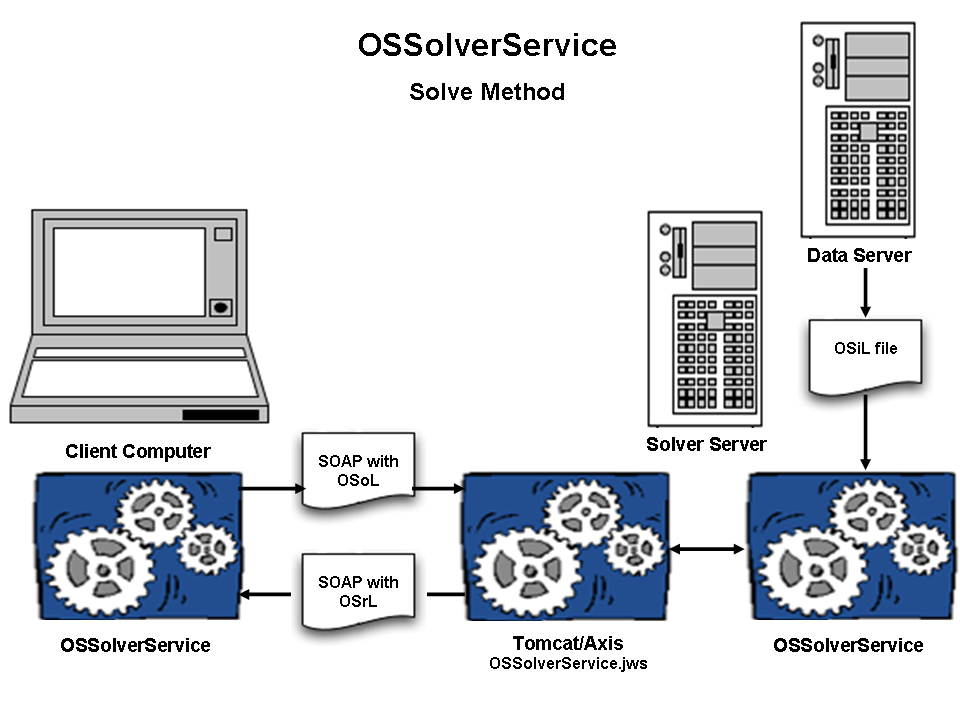
\includegraphics[scale=0.5]{./figures/Figure11.png}
\caption{Downloading the instance from a remote source.}
\label{figure:ossolverservice2}
\end{figure}

{\bf Note:} The {\tt solve} method communicates synchronously with the remote solver service
and once started, these jobs cannot be killed. This may not be desirable for large
problems when the user does not want to wait for a response or when there is a possibility
for the solver to enter an infinite loop. The {\tt send} service
method should be used when asynchronous communication is desired.\index{solve@{\tt solve}|)}


\subsubsection{The  {\tt send} Service Method}\label{section:send}

\index{send@{\tt send}|(}
When the {\tt solve} service method is used, then the {\tt OSSolverService} does not
finish execution until the solution is returned from the remote solver service.
 When the {\tt send}
method is used, the instance is communicated to the remote service and the
{\tt OSSolverService} terminates after submission. An example of this is
\begin{verbatim}
./OSSolverService config ../data/configFiles/testremoteSend.config
\end{verbatim}
where the {\tt testremoteSend.config} file is
\begin{verbatim}
-nl ../data/amplFiles/hs71.nl
serviceLocation http://kipp.chicagobooth.edu/os/OSSolverService.jws
serviceMethod send
\end{verbatim}
In this example the COIN-OR {\tt Ipopt}\index{COIN-OR projects!Ipopt@{\tt Ipopt}} solver is specified. The input file {\tt hs71.nl}
is in AMPL nl format\index{AMPL nl format|(}.
Before sending this to the remote solver service the {\tt OSSolverService} executable converts  
the nl format\index{AMPL nl format|)} into the OSiL\index{OSiL} XML format and packages this 
into the SOAP\index{SOAP protocol} envelope used by Web Services.

Since the {\tt send} method involves asynchronous communication the remote solver service must keep track of jobs.
The {\tt send} method requires a {\tt JobID}\index{JobID@{\tt JobID}|(}. In the above example no {\tt JobID} was specified.
When no {\tt JobID} is specified the {\tt OSSolverService} method first invokes the {\tt getJobID} service method
to get a {\tt JobID}, puts this information into an OSoL\index{OSoL|(} file it creates, and sends the information
to the server. More information on the {\tt getJobID} service method is provided in Section~\ref{section:getjobid}.
The {\tt OSSolverService} prints the OSoL file to standard output before termination.
This is illustrated below,

\begin{verbatim}
<?xml version="1.0" encoding="UTF-8"?>
<osol xmlns="os.optimizationservices.org"
      xmlns:xsi="http://www.w3.org/2001/XMLSchema-instance"
      xsi:schemaLocation="os.optimizationservices.org
      http://www.optimizationservices.org/schemas/2.0/OSiL.xsd">
    <general>
        <jobID>
            gsbrkm4__127.0.0.1__2007-06-16T15.46.46.075-05.00149771253
        </jobID>
        <solverToInvoke>ipopt</solverToInvoke>      
    </general>
</osol>
\end{verbatim}

The {\tt JobID} is one that is randomly generated by the server and passed back to the {\tt OSSolverService}.
The user can also provide a {\tt JobID} in their OSoL file. For example, below is a user-provided OSoL file that could
be specified in a configuration file or on the command line.

\begin{verbatim}
<?xml version="1.0" encoding="UTF-8"?>
<osol xmlns="os.optimizationservices.org"
      xmlns:xsi="http://www.w3.org/2001/XMLSchema-instance"
      xsi:schemaLocation="os.optimizationservices.org
      http://www.optimizationservices.org/schemas/2.0/OSiL.xsd">
    <general>
        <jobID>123456abcd</jobID>
        <solverToInvoke>ipopt</solverToInvoke>      
    </general>
</osol>
\end{verbatim}

The same {\tt JobID} cannot be used twice, so if {\tt 123456abcd} was used earlier, 
the result of {\tt send} will be an error condition\index{JobID@{\tt JobID}|)}.

In order to be of any use, it is necessary to get the result of the optimization. This is described in
Section~\ref{section:retrieve}. Before proceeding to this section, we describe two ways for knowing when
the optimization is complete. One feature of the standard OS remote SolverService is the ability to send an
email when the job is complete. Below is an example of the {\tt OSoL} that uses the email feature\index{OSoL|)}.

\begin{verbatim}
<?xml version="1.0" encoding="UTF-8"?>
<osol xmlns="os.optimizationservices.org"
      xmlns:xsi="http://www.w3.org/2001/XMLSchema-instance"
      xsi:schemaLocation="os.optimizationservices.org
      http://www.optimizationservices.org/schemas/2.0/OSiL.xsd">
    <general>
        <jobID>123456abcd</jobID>
        <contact transportType="smtp">
            kipp.martin@chicagogsb.edu
        </contact>
        <solverToInvoke>ipopt</solverToInvoke>      
    </general>
</osol>
\end{verbatim}

The remote Solver Service will send an email to the above address when the job is complete. A second option for
knowing when a job is complete is to use the {\tt knock}\index{knock@{\tt knock}} method.
(See Section~\ref{section:knock}.)

Note that in all of these examples we provided a value for the {\tt <solverToInvoke>} element.
%The remote solver service will use {\tt Cbc} if another solver is not specified.%
A default solver is used (see Table~\ref{table:defaultsolvers}\index{default solver}) if another solver is not specified.%
\index{send@{\tt send}|)}



\subsubsection{The  {\tt retrieve} Service Method}\label{section:retrieve}

\index{retrieve@{\tt retrieve}|(}
The {\tt retrieve} method is used to get information about the instance solution.  This method has a single string argument which is an OSoL instance. Here is an example of using the {\tt retrieve} method with {\tt OSSolverService}.
\begin{verbatim}
./OSSolverService config ../data/configFiles/testremoteRetrieve.config
\end{verbatim}
The {\tt testremoteRetrieve.config} file is
\begin{verbatim}
serviceLocation http://kipp.chicagobooth.edu/os/OSSolverService.jws
osol ../data/osolFiles/retrieve.osol
serviceMethod retrieve
osrl /home/kmartin/temp/test.osrl
\end{verbatim}
and the {\tt retrieve.osol} file is

\begin{verbatim}
<?xml version="1.0" encoding="UTF-8"?>
<osol xmlns="os.optimizationservices.org"
      xmlns:xsi="http://www.w3.org/2001/XMLSchema-instance"
      xsi:schemaLocation="os.optimizationservices.org
      http://www.optimizationservices.org/schemas/2.0/OSiL.xsd">
    <general>
        <jobID>123456abcd</jobID>
    </general>
</osol>
\end{verbatim}

The OSoL file {\tt retrieve.osol} contains a tag {\tt <jobID>} that is communicated to
the remote service. The remote service locates the result and returns it as a string.
The {\tt <jobID>}\index{JobID@{\tt JobID}} should reflect a {\tt <jobID>} that was previously submitted
using a {\tt send()} command.
The result is returned as a string in OSrL format.  The user must modify the line
\begin{verbatim}
osrl /home/kmartin/temp/test.osrl
\end{verbatim}
to reflect a valid path for their own machine.  (It is also possible to delete the line
in which case the result will be displayed on the screen instead of being saved to the
file indicated in the {\tt osrl} option.)\index{retrieve@{\tt retrieve}|)}


\subsubsection{The  {\tt getJobID} Service Method}\label{section:getjobid}

\index{getJobID@{\tt getJobID}|(}
Before  submitting a job with the {\tt send}\index{send@{\tt send}} method a {\tt JobID}\index{JobID@{\tt JobID}}
is required. The {\tt OSSolverService} can get a {\tt JobID} with the following options.
\begin{verbatim}
serviceLocation http://kipp.chicagobooth.edu/os/OSSolverService.jws
serviceMethod getJobID
\end{verbatim}
Note that no OSoL\index{OSoL} input file is specified. In this case, the {\tt OSSolverService} sends an empty string.
A string is returned with the {\tt JobID}. This {\tt JobID} is then put into a {\tt <jobID>} element in an
OSoL string that would be used by the {\tt send}\index{send@{\tt send}} method.
\index{getJobID@{\tt getJobID}|)}


\subsubsection{The  {\tt knock} Service Method}\label{section:knock}

\index{knock@{\tt knock}|(}
The OSSolverService terminates after executing the {\tt send}\index{send@{\tt send}} method. Therefore,
it is necessary to know when the job is completed on the remote server. One way is to include an email
address in the  {\tt <contact>}  element with the attribute {\tt transportType} set to {\tt smtp}.
This was illustrated in Section~\ref{section:solve}.  A second way to check on the status of a job is
to use the {\tt knock} service method.  For example, assume a user   wants to know if  the job
with {\tt JobID 123456abcd}\index{JobID@{\tt JobID}}  is complete. A user would make the request
\begin{verbatim}
./OSSolverService config ../data/configFiles/testRemoteKnock.config
\end{verbatim}
where the {\tt testRemoteKnock.config} file is
\begin{verbatim}
serviceLocation http://kipp.chicagobooth.edu/os/OSSolverService.jws
osplInput ../data/osolFiles/demo.ospl
osol ../data/osolFiles/retrieve.osol
serviceMethod knock
\end{verbatim}
the {\tt demo.ospl} file is

% header to be temporarily hidden...
% <ospl xmlns="os.optimizationservices.org">
%       xmlns:xsi="http://www.w3.org/2001/XMLSchema-instance"
%       xsi:schemaLocation="os.optimizationservices.org
%       http://www.optimizationservices.org/schemas/2.0/OSiL.xsd">

\begin{verbatim}
<?xml version="1.0" encoding="UTF-8"?>
<ospl xmlns="os.optimizationservices.org">
    <processHeader>
        <request action="getAll"/>
    </processHeader>
    <processData/>
</ospl>
\end{verbatim}
and the {\tt retrieve.osol} file is
\begin{verbatim}
<?xml version="1.0" encoding="UTF-8"?>
<osol xmlns="os.optimizationservices.org"
      xmlns:xsi="http://www.w3.org/2001/XMLSchema-instance"
      xsi:schemaLocation="os.optimizationservices.org
      http://www.optimizationservices.org/schemas/2.0/OSiL.xsd">
    <general>
        <jobID>123456abcd</jobID>
    </general>
</osol>
\end{verbatim}

The result of this request is a string in OSpL\index{OSpL|(} format, with the data contained in its
{\tt processData} section.  The result is displayed on the screen; if the user desires it
to be redirected to a file, a command should be added to the {\tt testRemoteKnock.config}
file with a valid path name on the local system, e.g.,

\begin{verbatim}
osplOutput ./result.ospl
\end{verbatim}

Part of the return format is illustrated below.

% Header to be temporarily hidden
% <ospl xmlns="os.optimizationservices.org"
%       xmlns:xsi="http://www.w3.org/2001/XMLSchema-instance"
%       xsi:schemaLocation="os.optimizationservices.org
%       http://www.optimizationservices.org/schemas/2.0/OSiL.xsd">

\begin{verbatim}
<?xml version="1.0" encoding="UTF-8"?>
<ospl xmlns="os.optimizationservices.org">
  <processHeader>
    <serviceURI>http://localhost:8080/os/ossolver/CGSolverService.jws</serviceURI>
    <serviceName>CGSolverService</serviceName>
    <time>2006-05-10T15:49:26.7509413-05:00</time>
  <processHeader>
  <processData>
     <statistics>
        <currentState>idle</currentState>
        <availableDiskSpace>23440343040</availableDiskSpace>
        <availableMemory>70128</availableMemory>
        <currentJobCount>0</currentJobCount>
        <totalJobsSoFar>1</totalJobsSoFar>
        <timeServiceStarted>2006-05-10T10:49:24.9700000-05:00</timeServiceStarted>
        <serviceUtilization>0.1</serviceUtilization>
        <jobs>
        <job jobID="123456abcd">
            <state>finished</state>
            <serviceURI>http://kipp.chicagobooth.edu/ipopt/IPOPTSolverService.jws</serviceURI>
            <submitTime>2007-06-16T14:57:36.678-05:00</submitTime>
            <startTime>2007-06-16T14:57:36.678-05:00</startTime>
            <endTime>2007-06-16T14:57:39.404-05:00</endTime>
            <duration>2.726</duration>
          </job>
        </jobs>
     </statistics>
  </processData>
</ospl>
\end{verbatim}
Notice that the {\tt <state>} element in {\tt <job jobID="123456abcd">} indicates that the job is finished.

When making a {\tt knock} request,  the OSoL string can be empty. In this example, if the OSoL string had been empty
the status of all jobs kept in the file ospl.xml is reported.  In our default solver service implementation,
there is a configuration file {\tt OSParameter} that has a parameter {\tt MAX\_JOBIDS\_TO\_KEEP }.
The current default setting is~100. In a large-scale or commercial implementation it might be wise to keep
problem results and statistics in a database. Also, there are values other than {\tt getAll} (i.e., get all
process information related to the jobs) for the OSpL {\tt action} attribute in the {\tt <request>} tag.
For example, the {\tt action} can be set to a value of {\tt ping} if the user just wants
to check if the remote solver service is up and running. For details, check the OSpL schema.\index{OSpL|)}
\index{knock@{\tt knock}|)}


\subsubsection{The  {\tt kill}   Service Method}

\index{kill@{\tt kill}|(}
If the user submits a job that is taking too long or is a mistake, it is possible to kill the job on the remote server using the {\tt kill} service method.
For example, to kill job {\tt 123456abcd}, at the command line type
\begin{verbatim}
./OSSolverService config  ../data/configFiles/kill.config
\end{verbatim}
where the configure file {\tt kill.config} is
\begin{verbatim}
osol ../data/osolFiles/kill.osol
serviceLocation http://kipp.chicagobooth.edu/os/OSSolverService.jws
serviceMethod kill
\end{verbatim}
and the {\tt kill.osol} file is
\begin{verbatim}
<?xml version="1.0" encoding="UTF-8"?>
<osol xmlns="os.optimizationservices.org"
      xmlns:xsi="http://www.w3.org/2001/XMLSchema-instance"
      xsi:schemaLocation="os.optimizationservices.org
      http://www.optimizationservices.org/schemas/2.0/OSiL.xsd">
    <general>
        <jobID>123456abcd</jobID>
    </general>
</osol>
\end{verbatim}

The result is returned in  OSpL format.
\index{kill@{\tt kill}|)}



\subsubsection{Summary and description of the API}

The six service methods just described are also available as callable routines.
Below is a summary of the inputs and outputs of the six methods. See also Figure~\ref{figure:osCommunicationMethods}.
A test program illustrating the use of the methods is described in Section~\ref{section:exampleOSRemoteTest}.

\begin{itemize}

\item {\tt solve( osil, osol ):}\index{solve@{\tt solve}}

\begin{itemize}

\item Inputs: a string with the instance in OSiL\index{OSiL} format and an optional string with the solver options
in OSoL\index{OSoL} format

\item Returns: a string with the solver solution in OSrL\index{OSrL} format

\item Synchronous call, blocking request/response

\end{itemize}



\item {\tt send( osil, osol ):}\index{solve@{\tt solve}}

\begin{itemize}

\item Inputs: a string with the instance in OSiL\index{OSiL} format and a string with the solver options
in OSoL\index{OSoL} format (same as in {\tt solve})

\item Returns:  %a boolean, true if the problem was successfully submitted, false otherwise
a string with the status of the send (indicating either success or some error condition).

\item Has the same signature as {\tt solve}

\item Asynchronous (server side), non-blocking call

\item The {\tt osol} string should have a {\tt JobID}\index{JobID@{\tt JobID}} in the {\tt <jobID>} element
\end{itemize}


\item {\tt getJobID( osol ):}\index{getJobID@{\tt getJobID}}

\begin{itemize}

\item Inputs: a string  with the solver options in OSoL\index{OSoL} format (in this case, the string
may be empty because no options are required to get the JobID)

\item Returns: a string which is the unique job id generated by the solver service

\item Used to maintain session and state on a distributed system
\end{itemize}



\item {\tt knock( ospl, osol ):}\index{knock@{\tt knock}}

\begin{itemize}

\item Inputs: a string in OSpL\index{OSpL} format and an optional string with the solver options in OSoL\index{OSoL} format

\item Returns: process and job status information from the remote server in OSpL format

\end{itemize}


\item {\tt retrieve( osol ):}\index{retrieve@{\tt retrieve}}

\begin{itemize}

\item Inputs: a string with the solver options  in OSoL\index{OSoL} format

\item Returns: a string with the solver solution in OSrL\index{OSrL} format

\item The {\tt osol} string should have a {\tt JobID}\index{JobID@{\tt JobID}} in the {\tt <jobID>} element

\end{itemize}


\item {\tt kill( osol ):}\index{kill@{\tt kill}}

\begin{itemize}

\item Inputs: a string with the solver options  in OSoL\index{OSoL} format

\item Returns: process and job status information from the remote server in OSpL\index{OSpL} format

\item Critical in long running optimization jobs

\end{itemize}

\end{itemize}
\index{OSSolverService@{\tt OSSolverService}|)}


\begin{figure}[ht]
\centering
%\includegraphics[scale=0.5]{\figurepath/osCommunicationMethods.pdf}
\includegraphics[scale=0.5]{./figures/osCommunicationMethods.pdf}
\caption{The OS Communication Methods}
\label{figure:osCommunicationMethods}
\end{figure}


\subsection{Passing Options to Solvers}

The OSoL (Optimization Services option Language) protocol is used to pass options to solvers.   
When using the {\tt OSSolverService} executable this will typically be done through an OSoL XML file 
by specifying the {\tt osol} option followed by the location of the file.  However, it is also possible 
to write a custom application that links to the OS library and to build an OSOption object in memory 
and then pass this to a solver. We next describe the  feature of the OSoL protocol that will be the most 
useful to the typical user.

In the OSoL protocol there is an element {\tt <solverOptions>} that can have any number of {\tt <solverOption>} 
children. (See the file {\tt parsertest.osol} in OS/data/osolFiles.)  Each {\tt <solverOption>} child can have 
six attributes, all of which except one are optional. These attributes are:

\begin{itemize}

\item {\bf name:} this is the only required attribute and is the option name. It should be unique.

\item {\bf value:}  the value of the option.

\item {\bf solver:} the name of the solver associated with the option. 
At present the values recognized by this attribute are 
{\tt "ipopt"}\index{COIN-OR projects!Ipopt@{\tt Ipopt}}, 
{\tt "bonmin"}\index{COIN-OR projects!Bonmin@{\tt Bonmin}}, 
{\tt "couenne"}\index{COIN-OR projects!Couenne@{\tt Couenne}}, 
{\tt "cbc"}\index{COIN-OR projects!Cbc@{\tt Cbc}}, 
and {\tt "osi"}\index{COIN-OR projects!Osi@{\tt Osi}|(}. 
The last option is used for all solvers that are accessed through the 
Osi interface, which are 
{\tt clp}\index{COIN-OR projects!Clp@{\tt Clp}},
 {\tt DyLP}\index{COIN-OR projects!DyLP@{\tt DyLP}}, 
{\tt SYMPHONY}\index{COIN-OR projects!SYMPHONY@{\tt SYMPHONY}} and 
{\tt Vol}\index{COIN-OR projects!Vol@{\tt Vol}}, in addition to 
{\tt Glpk}\index{Third-party software, {\tt GLPK}} and 
{\tt Cplex}\index{cplex@{\tt cplex}}, 
if the latter are included in the particular build of OSSolverService.
\index{COIN-OR projects!Osi@{\tt Osi}|)}

\item {\bf type:} this will usually be a data type (such as integer, string, double, etc.) but this is not necessary.

\item {\bf category:} the same solver option may apply in more than one context (and with different meaning) so it may be necessary
to specify a category to remove ambiguities. For example, in LINDO an option can apply to a specific model or to every model in an environment. 
Hence we might have

\begin{verbatim}
<solverOption name="LS_IPARAM_LP_PRINTLEVEL" 
   solver="lindo" category="model"  type="integer" value="0"/>
<solverOption name="LS_IPARAM_LP_PRINTLEVEL" 
   solver="lindo" category="environment" type="integer" value="1"/>
\end{verbatim}
where we specify the print level for a specific model or the entire environment.   The category attribute should be 
separated by a colon (`:') if there is more than one  category or  additional subcategories, 
as in the following hypothetical example.
\begin{verbatim}
<solverOption name="hypothetical" 
   solver="SOLVER" category="cat1:subcat2:subsubcat3" 
      type="string" value="illustration"/>
\end{verbatim}

\item {\bf description:} a description of the option; typically this would not get passed to the solver.

\end{itemize}

As of trunk version 2164\index{OS project!trunk version} the reading of an
OSoL file is implemented in the {\tt OSCoinSolver}, {\tt OSBonmin} and
{\tt OSIpopt} solver interfaces.   The  {\tt OSBonmin}, and {\tt OSIpopt}
solvers have particularly easy interfaces. They have methods for integer,
string, and numeric data types and then take options in form of
{\tt (name, value)} pairs. Below is an example of options for {\tt Ipopt}.


\begin{verbatim}
<solverOption name="mu_strategy" solver="ipopt" 
     type="string" value="adaptive"/>
<solverOption name="tol" solver="ipopt" 
     type="numeric" value="1.e-9"/>
<solverOption name="print_level" solver="ipopt" 
     type="integer" value="5"/>
<solverOption name="max_iter" solver="ipopt" 
     type="integer" value="2000"/>
\end{verbatim}

We have also implemented the {\tt OSOption} class for the {\tt OSCoinSolver} interface. This can be done in two ways. 
First, options can be set through the Osi Solver interface (the OSCoinSolver interface wraps around the Osi Solver interface).    
We have implemented all of the options listed in {\tt OsiSolverParameters.hpp} in {\tt Osi} trunk version 1316.  
In the Osi solver interface, in addition to string, double, and integer types  there is a type called {\tt HintParam}
and a type called {\tt OsiHintParam}. The value of the {\tt OsiHintParam} is an {\tt OsiHintStrength} type, 
which may be confusing. For example, to have the following Osi method called

\begin{verbatim}
setHintParam(OsiDoReducePrint, true, hintStrength);
\end{verbatim}


the user should set the following {\tt <solverOption>} tags:
\begin{verbatim}
<solverOption name="OsiDoReducePrint" solver="osi" 
    type="OsiHintParam"  value="true" />
<solverOption name="OsiHintIgnore" solver="osi" 
     type="OsiHintStrength" />
\end{verbatim}
There should be only one {\tt <solverOption>} with type {\tt OsiHintStrength} and if there are more than one in the 
OSoL file (string) the last one is the one implemented. 

In addition to setting options using the Osi  Solver interface, it is possible to pass options directly to the {\tt Cbc} 
solver. By default the following options are sent to the {\tt Cbc} solver,

\begin{verbatim}
-log=0  -solve 
\end{verbatim}
The option {\tt -log=0} will keep the branch-and-bound output to a minimum.  Default options are overridden by 
putting into the OSoL file at least one {\tt <solverOption>} tag with the {\tt solver} attribute 
set to {\tt cbc}.    For example, the following sequence of options will limit the search to 100 nodes, 
cut generation turned off.

\begin{verbatim}
<solverOption name="maxN" solver="cbc" value="100" />
<solverOption name="cuts" solver="cbc" value="off" />
<solverOption name="solve" solver="cbc"  />
\end{verbatim}

Any option that {\tt Cbc} accepts at the command line can be put into a {\tt <solverOption>} tag. We list  those below.

{\small
\begin{verbatim}
Double parameters:
  dualB(ound)  dualT(olerance)  primalT(olerance)  primalW(eight)  
Branch and Cut double parameters:
  allow(ableGap)  cuto(ff)  inc(rement)  inf(easibilityWeight)  integerT(olerance)  
  preT(olerance)  ratio(Gap)  sec(onds)  
Integer parameters:
  cpp(Generate)  force(Solution)  idiot(Crash)  maxF(actor)  maxIt(erations)  
  output(Format)  slog(Level)  sprint(Crash)  
Branch and Cut integer parameters:
  cutD(epth)  log(Level)  maxN(odes)  maxS(olutions)  passC(uts)  
  passF(easibilityPump)  passT(reeCuts)  pumpT(une)  strat(egy)  strong(Branching)  
  trust(PseudoCosts)  
Keyword parameters:
  chol(esky)  crash  cross(over)  direction  dualP(ivot)  
  error(sAllowed)  keepN(ames)  mess(ages)  perturb(ation)  presolve  
  primalP(ivot)  printi(ngOptions)  scal(ing)  
Branch and Cut keyword parameters:
  clique(Cuts)  combine(Solutions)  cost(Strategy)  cuts(OnOff)  Dins  
  DivingS(ome)  DivingC(oefficient)  DivingF(ractional)  DivingG(uided)  DivingL(ineSearch)  
  DivingP(seudoCost)  DivingV(ectorLength)  feas(ibilityPump)  flow(CoverCuts)  gomory(Cuts)  
  greedy(Heuristic)  heur(isticsOnOff)  knapsack(Cuts)  lift(AndProjectCuts)  local(TreeSearch)  
  mixed(IntegerRoundingCuts)  node(Strategy)  pivot(AndFix)  preprocess  probing(Cuts)  
  rand(omizedRounding)  reduce(AndSplitCuts)  residual(CapacityCuts)  Rens  Rins  
  round(ingHeuristic)  sos(Options)  two(MirCuts)  
Actions or string parameters:
  allS(lack)  barr(ier)  basisI(n)  basisO(ut)  directory  
  dirSample  dirNetlib  dirMiplib  dualS(implex)  either(Simplex)  
  end  exit  export  help  import  
  initialS(olve)  max(imize)  min(imize)  netlib  netlibD(ual)  
  netlibP(rimal)  netlibT(une)  primalS(implex)  printM(ask)  quit  
  restore(Model)  saveM(odel)  saveS(olution)  solu(tion)  stat(istics)  
  stop  unitTest  userClp  
Branch and Cut actions:
  branch(AndCut)  doH(euristic)  miplib  prio(rityIn)  solv(e)  
  strengthen  userCbc  
\end{verbatim}
}


The user may also wish to specify an initial starting solution. This is particularly
useful with interior point methods.  This is accomplished by using the
{\tt <initialVariableValues>} tag.  Below we illustrate how to set the
initial values for variables with an index of 0, 1, and~3.

\begin{verbatim}
<initialVariableValues numberOfVar="3">
   <var idx="0" value="1"/>
   <var idx="1" value="4.742999643577776" />
   <var idx="3" value="1.379408293215363"/>
</initialVariableValues>
\end{verbatim}

As of trunk version 2164\index{OS project!trunk version} the initial values for variables can be passed
to the {\tt Bonmin} and {\tt Ipopt} solvers.


When implementing solver options in-memory, the typical calling sequence is:

\begin{verbatim}
solver->buildSolverInstance();
solver->setSolverOptions();
solver->solve();
\end{verbatim}



